\documentclass[conference]{journal}

\title{Asignment Week 1}
\author{Nathan A. Nordby}

\usepackage{graphicx} %Loading the package 
\usepackage[space]{grffile} %Loading the package
\graphicspath{{/Users/Primary_User/Desktop/CS6000/figures/}} %Setting the graphicspath 
\usepackage{framed}
\usepackage{caption}
\usepackage{wrapfig}
\usepackage{float}
\usepackage{hyperref}

%\usepackage{biblatex}

%\addbibresource{references}


\begin{document}
\maketitle





\section{Introduction - Story and Goals}


\begin{wrapfigure}{L}{2cm}
\centering
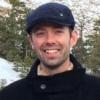
\includegraphics[width=0.125\textwidth]{Nathan.jpg}
\caption{\label{fig:Me} Me}
\end{wrapfigure}

	This semester I began CS6000 as a gift from Dr. Boult as a late add. I am very grateful that I was able to add the course. This semester my first and primary goal (I) is to be caught up as soon as reasonably posible . I also intend to use this course as a vehicle to: II) “get-good” at writing research papers and III) create a prototype design for a vehicle entry device I have been designing.  I am finishign up my MESE program this Spring 18' with an emphasis in security so that I can transition immediately into the PhD in Engineering - Concentration in Security.

\subsection{Catch-up}
It is my responsiblity to get caugt up and here is my plan: This is the first submission of 7 journals due. I intend to do 2 journals a week including this weekend, and the survey paper draft subnmitted by 19 Oct 18. Then I will submit the second survey paper draft by 26 Oct 18. So by 29 October I will be completely caught up with journals and other assignments.  I request instructor approval on this plan.

\subsection{Get-Goodness Factor}
Writing has been a significant challenge for me in my story: struggling in basics in grammar and writing and sometimes still surfaces. Homeschooled from 1st-4th grade included I lived through some significant personal family challenges. My mother noticed that I write “different”. From 5th grade to 9th grade I transitioned between three schools, public-charter-public. I landed in Highschool averaging C's and wondering why I couldn’t “get-good” grades. In 9th grade I gave my life to Jesus Christ-while dating a Christian girlfriend. The God of the Bible desires excellence and started to change me. Then, a Christian brother got me interested in The United States Air Force Academy (USAFA) in 9th grade. In high school I won state-level awards for oratory story-telling in speech. I think this gives some insight into how I write. My last year of high school with Gods help I finally had a good GPA. Now, I desire to clean-up some of these hitches in my get-up. This semester I intend to learn how to efficiently read research papers, understand the context of research paper writing, and then apply this to demonstrate an excellent research paper.
\subsection{Invent}
For a while I have been trying to create an alternate remote entry system for vehicles. I have worked the idea multiple times in my mind and being that I have done prototyping previously for the military and others I have decided to go forward with it; with a friend’s help. This semester I intend to use this course to read and understand (at the application level) as many good research papers as I can focusing on remote keyless entry systems for vehicles.

\section{ In the Bib-GIT-ing}
In the beginning of the semester for this course I had significant challenges personally and technically. I was finishing up a lengthy legal case that I ended up having to be pro-se on while registering for classes. After registering one of the classes was not possible due to my commute from Denver, and one instructor did not answer me for about two months. As a result, I had to find a class that would fill my requirements and be semi-remote. After entering this class late, additional issues came up from the previous legal matter. So, although I was able to review most of the material a month after class started I could not start the work. After the legal mater settled and catching up with my cryptography course I began the work. So my first challenge was overwhelming legal/personal matters and I overcame that by prayer and taking one thing at a time. My next challenge was technical. I had heard of LaTeX many times before and have written research papers but never with LaTeX. I primarily have a windows laptop for college, so it is not exactly the best command environment. It took me about 3-4 hours to get my head around what LaTeX was and why I also needed MiKTex, and BibTex (plus all the random packages from random repositories) and how that is going to interface with GIT hub. I used multiple you-tube videos, and stack exchange posts after going through the slides and intro material to get it all working. Although I am not at the 100 percent solution I would normally have achieved by using a word editor I have a “good-enough” for turn in solution. I inted to get OverLeaf working later. My repository is located here: 
\href{https://github.com/nathan-nordby/First.git}{https://github.com/nathan-nordby/First.git}

\section{Sample Survey of Remote Keyless Entry for Vehicles (RKE) Research}
In \cite{1386610} the authors discuss various attacks on vehicular RKE systems. Although the article is a little dated (2005) it establishes necessary basics still applicable today for successfully attacking and entering a vehicle without the RKE as designed. Specifically the authors discuss how there are five well known successful attacks: 1) Scan, 2) Playback, 3)Forward Detection, 4) Dictionary, and 5) Relay (Two-Thief Attack). Then these methods are down selected
\begin{wrapfigure}{r}{3cm}
\centering
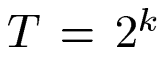
\includegraphics[width=0.125\textwidth]{Equation1.png}
\caption{\label{fig:Equation1} Equation 1}
\end{wrapfigure}
 based on their difficulty in successful implementation against RKE types (fixed code, rolling code, challenge-response, and another protocol) and difficulty in technological implementation.  As a result of this analysis the authors demonstrate and focus on the use of a Dictionary attack on a Challenge-Response RKE since it is the 
\begin{wrapfigure}{l}{3cm}
\centering
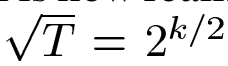
\includegraphics[width=0.125\textwidth]{Equation2.png}
\caption{\label{fig:Equation2} Equation 2}
\end{wrapfigure}

easiest to implement and Challenge-Response is the most difficult capability to attack. The authors use basics in cryptography to establish (eq1) that the basic key search space is relative to time is:  where k is the key length in bits. Then using this attack they try to minimize the time it takes for an attacker to build the necessary dictionary for a successful attack (eq 2)  . 
\begin{wrapfigure}{r}{3cm}
\centering
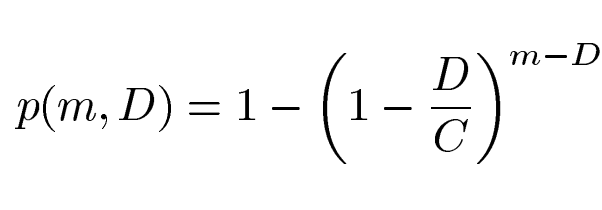
\includegraphics[width=0.5\textwidth]{Equation3.png}
\caption{\label{fig:Equation3} Equation 3}
\end{wrapfigure}
   Therefore the authors introduce (eq3) with ‘m’ trials where the probability of the attack is considered in likeliness for success.  
\begin{wrapfigure}{r}{3cm}
\centering
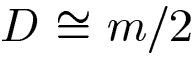
\includegraphics[width=0.125\textwidth]{Equation4.png}
\caption{\label{fig:Equation4} Equation 4}
\end{wrapfigure}
Since depending on k this can be a very large dictionary requiring significant time and hardware they use average cases of attack to do equivalently a ‘brute force’ attack using pdfs and cdfs. Therefore, the number of trials will be roughly half the size of the dictionary dependent on the k bit key size. The authors further reduce and differentiate the original equations to arrive on their final equation of (eq4) where this will maximize the likeliness of success to demonstrate this concept. This lines up with traditional cryptographic research where an average brute force attack usually requires half of the search space to be successful. 
In \cite{1624023} the authors discuss practical methods they tested to attack proximity RFIDs using eavesdropping to copy the signal and then later spoof it to deceive the control system. The authors provide actual distances and delays required to active and rx/tx data from to RFIDs along with spectral analysis of the work they did. In \cite{6234155} The authors discuss a protective algorithm they designed to prevent relay attacks against passive keyless entry systems for vehicles. They claim to have designed a better protocol than most only using 2n bits of memory. In \cite{7223297} the authors discuss how the automotive industry is in competition to have the most "connected" system. As a result, they have created multiple under the hood connections to the vehicle directly and now require layered internet security since they are ultimately vulnerable to remote attack. In \cite{7991092} the authors discuss the protocol implementation and potential design of Secret Unknown Ciphers (SUC) for vehicles using Physical Unclonable Functions (PUFs). PUFs are based on the physical identity of the microdevice optical or silicon properties serving inherently as a unique DNA for each manufactured device.

\section{References}

\bibliography{/Users/Primary_User/Desktop/CS6000/references}
\bibliographystyle{IEEEtran}

%\printbibliography
\end{document}